\reading{LTR-15}{The US Dollar Shortage in Global Banking and the International Policy Response}{DEFER}{0}
\markboth{LTR-15\ \ The US Dollar Shortage in Global Banking}{}

\begin{lrkeybox}[Learning objectives — official 2026 spine wording]
\begin{enumerate}[label=\textbf{\alph*.}]
\item Identify the causes of the U.S. dollar shortage during the Great Financial Crisis.
\item Evaluate the importance of assessing maturity/currency mismatches across the balance sheets of consolidated entities.
\item Describe the policy response by international central banks to alleviate the U.S. dollar shortage and assess its effectiveness.
\end{enumerate}
{\footnotesize\color{FRMGrey}Source: Patrick McGuire and Goetz von Peter, ``The US Dollar Shortage in Global Banking and the International Policy Response,'' BIS Working Papers, 2009.}
\end{lrkeybox}

\begin{lrtrapbox}[Ordering and stale wording]
The Crash layer presents these objectives as \textbf{b, a, c}, with a and c under a merged heading; they are resequenced here. Both layers also render objective \textbf{c} as ``\emph{Discuss how central bank swap agreements overcame challenges commonly associated with international lenders of last resort}''. The 2026 spine is broader: ``\emph{Describe the policy response by international central banks\ldots \textbf{and assess its effectiveness}}''. The assessment half is examinable and the notes' wording obscures it.
\end{lrtrapbox}

% =====================================================================
\lo{LTR-15 a}{Identify the causes of the U.S. dollar shortage during the Great Financial Crisis.}

\begin{center}
\small
\begin{tabularx}{\textwidth}{@{}p{0.5cm} X@{}}
\toprule
\rowcolor{FRMSoft}\textbf{\#} & \textbf{Cause} \\
\midrule
1 & The funding difficulties that arose during the crisis are \textbf{directly linked to the remarkable expansion in banks' global balance sheets} over the preceding decade. \\
\addlinespace
2 & The \textbf{accumulation of US dollar assets} saddled banks with significant funding requirements, which they scrambled to meet during the crisis --- via cross-currency funding, and revealed as banks' \textbf{US dollar funding gap}. \\
\addlinespace
3 & Funding risk hinges on the degree of \textbf{maturity transformation} embedded in banks' balance sheets. Banks increasingly funded \textbf{long-term US dollar assets with short-term liabilities}, producing significant funding gaps when those liabilities needed rolling over into a stressed market. \\
\addlinespace
4 & Events during the crisis severely disrupted banks' sources of short-term funding. \textbf{Interbank markets seized up}, and \textbf{dislocations in FX swap markets} made it more expensive to obtain US dollars via swaps, as counterparty risk rose and liquidity shortages spread. \\
\addlinespace
5 & Banks have become so globalised, with offices in many countries, that it is \textbf{impossible to identify vulnerabilities in their balance sheets using residency-based statistics alone}. \\
\bottomrule
\end{tabularx}
\end{center}

\begin{lrkeybox}[Two further pressures named in the Crash layer]
\begin{itemize}
\item \textbf{Money markets reduced their exposure} to bank-issued securities, and \textbf{central banks decreased their US dollar reserves}, further straining dollar liquidity.
\item Banks \textbf{struggled to sell US dollar assets without incurring losses}, except for highly liquid US government securities. Pre-crisis \textbf{off-balance-sheet vehicles were re-integrated} into banks' balance sheets, increasing the demands on liquidity.
\end{itemize}
\end{lrkeybox}

\begin{lrtrapbox}[The shortage was a funding-structure problem, not a solvency problem]
Every cause on the list is about \textbf{where the dollars came from and how long they lasted}, not about the credit quality of the dollar assets themselves. The reading's own conclusion --- cause 5 --- is methodological: residency-based statistics cannot see the vulnerability, which is why the next objective exists.
\end{lrtrapbox}

% =====================================================================
\lo{LTR-15 b}{Evaluate the importance of assessing maturity/currency mismatches across the balance sheets of consolidated entities.}

\subsection{Before the crisis, 2000--2007}

\begin{itemize}
\item Banks dramatically increased their global investments, especially in US dollars and structured products. Between 2000 and 2007 banks' \textbf{foreign claims more than tripled}, with \textbf{US dollar claims a major driver} of the growth.
\item Funding came from \textbf{three sources}: borrowing domestic currency and converting it to US dollars; using \textbf{FX swaps} to convert domestic currency to US dollars; and borrowing US dollars directly.
\item This exposed banks to \term{funding risk} --- the risk of not being able to roll over maturing liabilities.
\end{itemize}

\begin{lrkeybox}[Funding patterns differed by region]
\begin{itemize}
\item \textbf{Europe:} primarily funded foreign claims with \textbf{domestic} currency.
\item \textbf{Other countries:} funded foreign claims with \textbf{foreign} currencies, mostly US dollars.
\end{itemize}
The European pattern created \textbf{long foreign currency positions funded by short-term domestic currency borrowing} --- a currency mismatch layered on top of a maturity mismatch.
\end{lrkeybox}

\subsection{Why foreign currency mismatch was the concern}

\begin{itemize}
\item \textbf{Assets had longer maturities than liabilities} --- the funding gap. If banks could not roll over liabilities, they would have to sell assets, potentially at a loss.
\item \textbf{Domestic funding risk was lower}, because central banks could provide emergency liquidity in their own currency. Foreign currency funding had no such backstop --- which is the whole reason the policy response in objective c had to take the form it did.
\item \textbf{Transparency issue.} Banks did not disclose details of their international positions, making vulnerabilities hard to assess.
\end{itemize}

\begin{lrtrapbox}[Domestic and foreign funding risk are not symmetric]
A central bank can create its \emph{own} currency and cannot create dollars. That asymmetry is the reading's central point, and it is what a distractor treating the two funding risks as equivalent destroys.
\end{lrtrapbox}

\subsection{Why foreign offices matter}

\begin{enumerate}[label=\alph*)]
\item Large banks operate globally, so mismatches can occur at \textbf{individual offices}.
\item These mismatches \textbf{might be offset across different offices}, creating a hedged position overall.
\item Foreign offices book a \textbf{large share} of banks' foreign currency claims.
\item \textbf{Bank nationality does not necessarily reflect risk} --- look at the \textbf{global consolidated balance sheet}.
\item Banks' decisions about where to locate foreign offices can significantly impact foreign countries' external positions.
\end{enumerate}

\subsection{Maturity mismatches}

\begin{itemize}
\item It is difficult to get an accurate picture of the maturity of foreign currency assets and liabilities.
\item \textbf{BIS data on counterparty sectors} helps assess US dollar funding gaps.
\item \textbf{Funding gaps are the difference between long-term US dollar assets and long-term US dollar liabilities.}
\item The maturity of liabilities from different counterparties creates a \textbf{range} for the funding gap estimate --- which is why the figure is given as a band, not a point.
\item \textbf{By 2007, European banks had a US dollar funding gap estimated at \$1--2.2 trillion}, and relied on interbank markets, central banks and FX swaps to meet their funding needs.
\end{itemize}

\begin{lrtrapbox}[Consolidated, not residency-based — and it is a range]
Two precise points carry this objective. First, the unit of analysis is the \textbf{global consolidated balance sheet}, not the bank's nationality or the residency of the booking office. Second, the \$1--2.2 trillion figure is a \textbf{range} arising from uncertainty about counterparty maturities; an option quoting it as a single number has lost the reason the range exists.
\end{lrtrapbox}

% =====================================================================
\lo{LTR-15 c}{Describe the policy response by international central banks to alleviate the U.S. dollar shortage and assess its effectiveness.}

\begin{lrkeybox}[The swap line network]
Major central banks, led by the \textbf{Federal Reserve}, created a network of \textbf{swap lines}. These allowed other central banks to \textbf{borrow US dollars from the Fed in exchange for their own currencies}, and then provide those dollars to banks in their own jurisdictions.

The network \textbf{initially involved European and Swiss central banks} and \textbf{expanded to include others}. In \textbf{late 2008 the Fed made the swaps unlimited}, stabilizing markets.
\end{lrkeybox}

\begin{center}
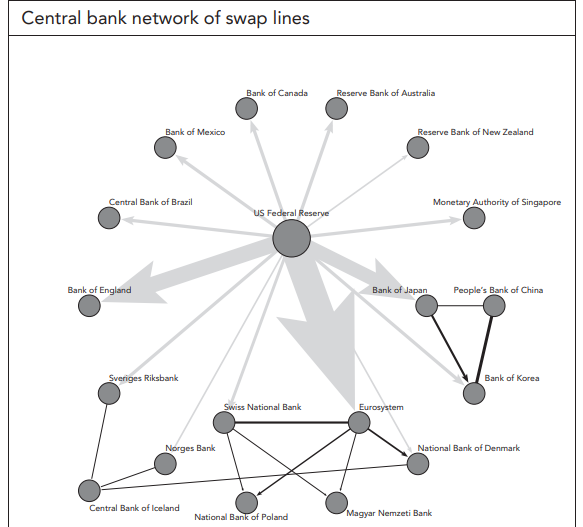
\includegraphics[width=0.62\textwidth]{fig/swaplines.png}
\figcap{The central bank network of swap lines, reproduced from the source notes (source: central banks). The Fed sits at the hub with every arrow originating from it; arrow thickness indicates the size of the line, with the \textbf{Eurosystem, Bank of England and Swiss National Bank} the heaviest. Note the secondary structures at the edges --- Japan--China--Korea, and the Nordic and central European cluster around the Eurosystem --- which are swap lines \emph{between} other central banks, not with the Fed. A hub-and-spoke network with regional sub-networks, not a single ring.}
\end{center}

\subsection{Assessing effectiveness}

\begin{center}
\small
\begin{tabularx}{\textwidth}{@{}p{4.6cm} X@{}}
\toprule
\rowcolor{FRMSoft}\textbf{Benefit} & \textbf{Mechanism} \\
\midrule
\textbf{Provided US dollar liquidity to banks globally} & Dollars reached banks that had no direct access to the Fed, through their own central banks. \\
\addlinespace
\textbf{Reduced pressure on the US dollar's value} & Demand that would otherwise have been met in the market was met by the Fed directly. \\
\addlinespace
\textbf{Mitigated pressure on other currencies} & Because of the Fed's ability to create more dollars, other central banks did not have to sell reserves or their own currencies to obtain them. \\
\addlinespace
\textbf{Avoided moral hazard} & The swap lines were \textbf{collateralized} --- the borrowing central bank posts its own currency --- which reduced risk for the Fed. \\
\addlinespace
\textbf{Reduced interbank rate volatility} & Observed effect once the swaps were made unlimited in late 2008. \\
\bottomrule
\end{tabularx}
\end{center}

\begin{lrtrapbox}[Why the moral hazard point is the subtle one]
An international lender of last resort normally raises two objections: who bears the credit risk, and whether the facility encourages the behaviour that created the problem. The swap structure answers both with one feature --- the arrangement is \textbf{collateralized in the borrowing central bank's own currency}, so the Fed's counterparty is a central bank, not a commercial bank, and the credit risk is on a sovereign monetary authority. A statement claiming the swap lines increased moral hazard, or that they were uncollateralized, inverts the reading's assessment.
\end{lrtrapbox}

\begin{lrtrapbox}[Consolidated trap summary — LTR-15]
\begin{itemize}
\item \textbf{Scope.} The dollar shortage was a \textbf{funding-structure} problem: long dollar assets, short non-dollar liabilities.
\item \textbf{Role.} \textbf{Europe} funded foreign claims with \emph{domestic} currency; other regions used \emph{foreign} currency, mostly dollars.
\item \textbf{Polarity.} Domestic funding risk was \textbf{lower} because the central bank can supply its own currency; foreign currency funding had no domestic backstop.
\item \textbf{Scope.} Assess vulnerability on the \textbf{global consolidated balance sheet}. Bank nationality and residency-based statistics do not reveal it.
\item \textbf{Definition.} The US dollar funding gap $=$ long-term dollar assets minus long-term dollar liabilities. The \textbf{\$1--2.2 trillion} figure is a \emph{range}, because counterparty maturities are uncertain.
\item \textbf{Role.} Swap lines run \textbf{Fed $\rightarrow$ other central banks $\rightarrow$ local banks}. The Fed's counterparty is a central bank, never a commercial bank.
\item \textbf{Scope.} \textbf{Collateralized}, and therefore \textbf{moral-hazard avoiding} --- the opposite of the usual objection to a lender of last resort.
\item \textbf{Definition.} The swaps became \textbf{unlimited in late 2008}; that is the point at which markets stabilized and interbank rate volatility fell.
\end{itemize}
\end{lrtrapbox}
